


%================================================================
\chapter{Simulation-Based Inference}\label{chap:LFI}
%================================================================

Intro, models without an explicit likelihood function, how to do Bayesian inference?

Simulation-based inference is also known as LFI, however we prefer the former as the latter indicates that the likelihood is not present at all, which we will see is not the case. Simulation-based, or "likelihood-free", inference algorithms only circumvent explicit evaluations of the likelihood. 

Something about ABC

\section{Likelihood-Based vs. Likelihood-Free}

Suppose a data-generating process is controlled by parameters $\theta$. When the process is run forward it stochastically generates a datapoint $y$ whose distribution depends on $\theta$. For every setting of $\theta$, assume that the process defines a conditional density function $\lhood$. Given an observed datapoint $y_0$ known to be generated by the process, the problem of interest is inferring plausible parameter settings that could have generated $y_0$. In particular, computing the posterior density $\pi \qty(\theta \mid y=y_0)$ obtained by Bayes theorem (\autoref{eq:bayes_theorem}) is of interest. The choice of inference algorithm primarily depends on how the data-generating process is modelled.
%\cite[p. 54]{papamakarios2019neural}. 

A purely statistical model, also known as a \textit{density model} or \textit{explicit model}, describes the conditional density function $\lhood$ of the process given values for $y$ and $\theta$. With a density model, the posterior density $\pi \qty(\theta \mid y=y_0)$ is, in general, easily evaluated using Bayes theorem. Even though the normalizing constant (or evidence) $p\qty(y_0)$ is typically intractable, samples from the posterior can be generated using a number of popular algorithms such as importance sampling and Markov chain Monte Carlo, or the posterior can be approximated with a more convenient distribution using e.g. variational inference. Such methods are referred to as \textit{likelihood-based inference methods}, as they explicitly evaluate the likelihood $\lhood$.
%\cite[p. 55]{papamakarios2019neural} \cite[p. 4]{abc_handbook}.

On the contrary, a \textit{simulator model}, also known as an \textit{implicit model}, describes how the process generates data. Many mechanical models are implicitly defined through simulator models, that is, as a set of dynamical equations and possibly a description of stochastic processes. For any parameter setting $\theta$, a simulator model can be run forward to generate independent samples from $\lhood$. Unlike for explicit density models, likelihoods are generally intractable or computationally infeasible for complex data-generating processes such as simulation-based models. The absence or complexity of the associated likelihood typically arise from it involving computationally expensive or intractable integrals, or that the simulator's internal states are unavailable. In order to perform inference in a simulator model, methods using simulations from the model rather than likelihood evaluations are needed. Such methods are referred to as \textit{likelihood-free inference methods}.
%\cite{SNL18} \cite{SNPE17} \cite[p. 55]{papamakarios2019neural}.

In general, likelihood-free methods are less efficient than likelihood-based methods as the former can require lots of simulations to produce accurate results. One of the principal topics of research in likelihood-free inference is how to obtain state-of-the-art results with fewer simulations. 
%\cite{comparison_snl_snpe}. 

%================================================================
\section{Approximate Bayesian Computation}\label{sec:abc}
%===============================================================

Approximate Bayesian Computation (ABC) constitutes a class of computational methods rooted in Bayesian statistics that can be used to evaluate posterior distributions of model parameters without having to explicitly calculate likelihoods. ABC methods approximate the likelihood function by assessing how likely it is the model could have produced the observed data, based on comparing synthetic data generated by the simulator to the observed data. The simulations that do not reproduce the observed data within a specified tolerance are discarded \cite{ABCprimer}.
%\cite[p. ix]{abc_handbook}.

ABC methods have been successfully applied to a wide range of real-world problems, and have also paved the way for a range of other likelihood-free approaches. However, even though ABC methods are mathematically well-founded, they inevitably make assumptions and approximations whose impact needs to be carefully assessed \cite{ABCprimer}. In the following, three types of ABC methods will be discussed: the vanilla \textit{rejection ABC}, and the more sophisticated variant \textit{Markov chain Monte Carlo (MCMC) ABC}.


%================================================================
\subsection{Rejection ABC}\label{sec:rejection_abc}
%================================================================

Given observed data $y_0$ and synthetic data $y$ generated by a simulator, let $\rho (\cdot, \cdot)$ be a distance metric (e.g., the Euclidean norm) defined in data space $\R^D$ and $\epsilon \geq 0$ be a tolerance. For small $\epsilon$, the ABC approximation to the posterior is 

\begin{equation}
    \pi \qty(\theta \mid y=y_0) \simeq \pi \qty(\theta \mid \rho \qty(y, y_0) \leq \epsilon)
\end{equation}


Rejection ABC is a rejection-sampling method for obtaining independent samples from the approximate posterior $ \pi \qty(\theta \mid \rho \qty(y, y_0) \leq \epsilon)$. It works by first sampling a set of parameters from the prior $\prior$, then simulating data under the model specified by the sampled parameters, and only accepting and retaining the sample if the distance between $y$ and $y_0$ is no more than $\epsilon$. The tolerance parameter $\epsilon$ controls the trade-off between estimation accuracy and computational efficiency. With sufficiently small $\epsilon$, and a sensible distance metric, the accepted samples follow the exact posterior more closely, though the algorithm accepts less often. On the other hand, the algorithm accepts more often with a large $\epsilon$, but the accepted samples will yield a replica of the prior.
%\cite[p. 58]{papamakarios2019neural} \cite{abc_handbook}. 

An issue with ABC in general is that the required number of simulations increases dramatically as $\epsilon$ becomes small. Moreover, likelihood-free inference also becomes challenging when the dimensionality of the data is large. A common approach to lessen this problem is to use lower-dimensional summary statistics, $S(y)$ and $S(y_0)$, that capture important features such as the mean and standard deviation, in place of raw data. %\cite{SNL18}. 
A further motivation for this approach is that real-world experiments often are interested in capturing summary statistics of the experimental data. A summary statistic that contains the same amount of information about model parameters as the whole dataset, is referred to as being a \textit{sufficient statistic} \cite{ABCprimer}. The acceptance criterion in the rejection ABC algorithm then becomes:

\begin{equation}
    \rho \qty(S(y), S(y_0))
\end{equation}

In \autoref{fig:abc_pipeline}, a conceptual overview of the rejection ABC algorithm is shown. 

\begin{figure}[H]
    \centering 
    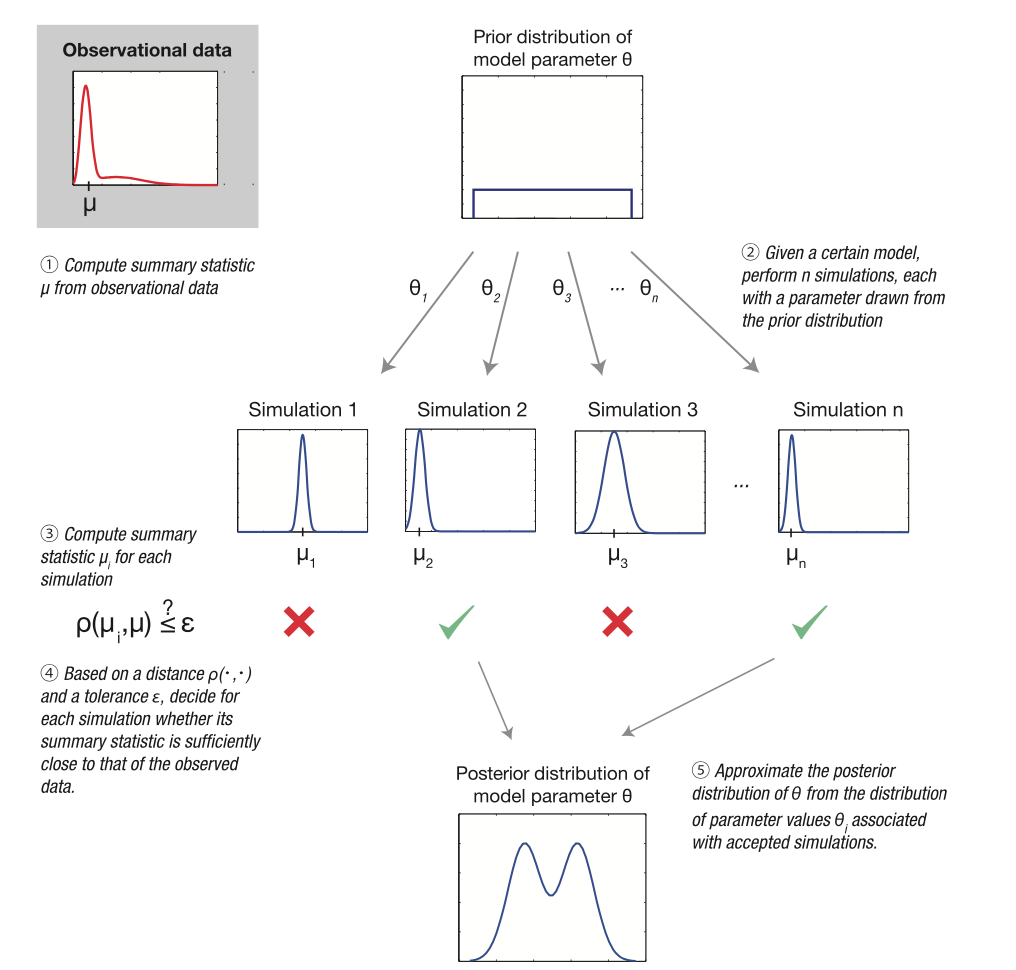
\includegraphics[scale=0.7]{./3_Images/abc_pipeline.png}
    \caption{Parameter estimation by Approximate Bayesian Computation: a conceptual overview.}
    \source{Figure 1 in \cite{ABCprimer}}
    \label{fig:abc_pipeline}
\end{figure}


\begin{algorithm}[H]
\caption{Rejection ABC}
\label{alg:mcmcabc}
\SetAlgoLined
\DontPrintSemicolon
 % Algorithm 
 \textbf{Inputs\,:}\;
 \vspace{-5mm}
 \begin{itemize}
     \item A target posterior density $\posterior \propto \lhood \prior$ consisting of a prior $\prior$ and likelihood $\lhood$. 
     \item A symmetric Markov proposal density $q \qty(\theta^* \mid \theta)$.
     \item An integer $N>0$.
 \end{itemize}
 
 \vspace{5mm}
 \textbf{Initialize\,:}\;
 Sample $\theta_0 \sim \prior$.\;

 \vspace{5mm}
 \textbf{Sampling\,:}\;
 \For{$t=1, ..., N$}{ 
 Generate proposal $\theta^* \sim q \qty(\theta^* \mid \theta_{t-1})$. \; 
 Calculate acceptance criterion $\alpha = \min \qty(1, \dfrac{p \qty(y \mid \theta^*) \pi \qty(\theta^*)}{p \qty(y \mid \theta_{t-1}) \pi \qty(\theta_{t-1})})$. \;
 Sample $u \sim \mathrm{U}(0,1)$. \; 
 \vspace{2mm}
 \eIf{$u \leq \alpha$}{
   $\theta_t = \theta^*$\;
   }{
   $\theta_t = \theta_{t-1}$\;
  }
 }
\end{algorithm}


%================================================================
\subsection{Markov Chain Monte Carlo ABC}\label{sec:mcmc_abc}
%================================================================

In the rejection ABC algorithm, parameters are sample from the prior $\prior$, and only parameters that are likely under the approximate posterior $\pi \qty(\theta \mid \rho \qty(y, y_0 ) \leq \epsilon )$ are accepted. The acceptance rate will be low if the approximate posterior is significantly narrower than the prior, as is often the case. %\cite[p. 59]{papamakarios2019neural}.

Markov-chain Monte Carlo (MCMC) ABC is an alternative approach that can lead to fewer rejections. Instead of proposing parameters from the prior, this method use the Metropolis-Hastings algorithm to propose new parameters $\theta'$ based on previously accepted parameters $\theta$ from the proposal density $q \qty(\theta' \mid \theta)$. By calculating the \textit{acceptance ratio}

\begin{equation}
    \alpha = \frac{p \qty(\rho \qty(y, y_0 ) \leq \epsilon \mid \theta') \pi\qty(\theta') q \qty(\theta \mid \theta')  }{p \qty(\rho \qty(y, y_0) \leq \epsilon \mid \theta) \pi\qty(\theta) q \qty(\theta' \mid \theta) },
\end{equation}

the algorithm outputs the proposed parameters $\theta'$ with probability $\min \qty(1, \alpha)$, otherwise it outputs the previous parameters $\theta$. 
%\cite[p. 59]{papamakarios2019neural}.

The approximate likelihood $p \qty(\rho \qty(y, y_0 ) \leq \epsilon \mid \theta)$ cannot be directly evaluated in the likelihood-free situation, but it can be estimated as the fraction of the simulated data $y$ whose distance from the observed data $y_0$ is no more than $\epsilon$:

\begin{equation}
    p \qty(\rho \qty(y, y_0) \leq \epsilon \mid \theta) \approx \frac{1}{N} \sum_n I \qty(\rho \qty(y_n, y_0) \leq \epsilon),
\end{equation}

where $y_n \sim p \qty(y \mid \theta)$ and $I(\cdot)$ is an indicator function. %\cite[p. 59]{papamakarios2019neural}.

Similarly to rejection ABC, the acceptance probability of MCMC ABC decreases as $\epsilon$ becomes small. Moreover, the performance of MCMC ABC strongly depends on the selection of proposal and prior density.

\begin{algorithm}[H]
\caption{Markov chain Monte Carlo ABC}
\label{alg:mcmcabc}
\SetAlgoLined
\DontPrintSemicolon
 % Algorithm 
 \textbf{Inputs\,:}\;
 \vspace{-5mm}
 \begin{itemize}
     \item A target posterior density $\posterior \propto \lhood \prior$ consisting of a prior $\prior$ and likelihood $\lhood$. 
     \item A symmetric Markov proposal density $q \qty(\theta^* \mid \theta)$.
     \item An integer $N>0$.
 \end{itemize}
 
 \vspace{5mm}
 \textbf{Initialize\,:}\;
 Sample $\theta_0 \sim \prior$.\;

 \vspace{5mm}
 \textbf{Sampling\,:}\;
 \For{$t=1, ..., N$}{ 
 Generate proposal $\theta^* \sim q \qty(\theta^* \mid \theta_{t-1})$. \; 
 Calculate acceptance criterion $\alpha = \min \qty(1, \dfrac{p \qty(y \mid \theta^*) \pi \qty(\theta^*)}{p \qty(y \mid \theta_{t-1}) \pi \qty(\theta_{t-1})})$. \;
 Sample $u \sim \mathrm{U}(0,1)$. \; 
 \vspace{2mm}
 \eIf{$u \leq \alpha$}{
   $\theta_t = \theta^*$\;
   }{
   $\theta_t = \theta_{t-1}$\;
  }
 }
\end{algorithm}

%================================================================
\subsection{Sequential Monte Carlo ABC}\label{sec:smc_abc}
%================================================================

TODO

%================================================================
\subsection{Population Monte Carlo ABC}\label{sec:pmc_abc}
%================================================================

TODO

\section{Notes}

\begin{itemize}
    \item See LFI for cognitive science book, Ch. 2.1
\end{itemize}

\textbf{Snippets:}

Although the steps listed above may give the impression that all likelihood- free algorithms are simple, this is unfortunately not the case. Many sophisticated techniques have been created in the hopes of increasing the efficiency of an algorithm on a given problem, and as one might expect, the efficiency of the algorithms below do vary by the type of problem to which they are applied. Because the algorithms we present later in this chapter are sometimes complex, we first introduce a few concepts at a high level by describing the different choices one can make at Steps 1, 2, or 3. 

The ABC methodology, where ABC stands for approxi- mate Bayesian computation, was mentioned as early as 1984 through a pedagogical and philosophical argument in Rubin (1984). It offers an almost automated resolution of the dif- ficulty with models which are intractable but can be simu- lated from. It was first proposed in population genetics by Tavaré et al. (1997), who introduced Approximate Bayesian Computation methods as a rejection technique bypassing the computation of the likelihood function via a simulation from the corresponding distribution. The exact version of the method can only be implemented in a small range of cases. Pritchard et al. (1999) produce a generalisation based on an approximation of the target. We study here the foundations as well as the implementation of the ABC method, with il- lustrations from time series. 

\textbf{Books/papers:} 

\begin{itemize}
    \item marin2012\_article\_abc, bra abc analyser 
\end{itemize}

LFI chapter, 2019 book statistics and data science, side 98, ligning (2): 

Unfortunately, we cannot evaluate (2) explicitly. However it is possible to drawn an IID random sample $T_N = \{ \Theta_j \}_{j=1}^N$ $(N \in \mathbb{N})$ from the quasi-posterior distribution that is characterized by (2), using the so-called rejection algorithm. 

\textbf{Links:}

\url{https://www.ncbi.nlm.nih.gov/pmc/articles/PMC4297650/}

Clearly, deciding how to characterize the data is an important choice in the likelihood-free context. Namely, it is impossible to know whether or not a set of statistics is sufficient for the unknown parameters if the likelihood is intractable.

\url{https://github.com/bmorris3/abc_interact/blob/master/abc_interact.ipynb}

\url{https://github.com/elfi-dev/elfi/blob/dev/elfi/methods/parameter_inference.py}

\textbf{MCMC} 

\url{https://github.com/davidtgonzales/ABC/blob/master/Lotka-Volterra%20ABC.ipynb}

\textbf{SMC} 

\url{https://docs.pymc.io/notebooks/SMC-ABC_Lotka-Volterra_example.html}

\url{https://github.com/pymc-devs/pymc3/tree/master/pymc3/smc}

\url{https://github.com/ICB-DCM/pyABC/blob/main/pyabc/inference/smc.py}

\url{https://github.com/vuolleko/abclib/blob/master/abclib.pyx}

\url{https://github.com/Neojume/pythonABC/blob/master/algorithms.py}


%================================================================
\section{The ABC of Approximate Bayesian Computation}\label{sec:abc_of_abc}
%================================================================

Content from notebook, source: ABC handbook

For discrete data $\mathcal{D}$, probability model $\mathcal{M}$ with parameters $\theta$ having prior $\pi(\theta)$, we can simulate observations from: 

\begin{equation}
    \pi (\theta \mid \mathcal{D}) \propto p(\mathcal{D} \mid \theta) \pi(\theta),
\end{equation}

via:

\begin{itemize}
    \item[A1] Generate $\theta \sim \pi(\theta)$
    \item[A2] Accept $\theta$ with probability proportional to the likelihood $p(\mathcal{D}\mid \theta)$
\end{itemize}
    
Algorithm A can be extended dramatically in its usefulness using the following, stochastically equivalent, version:

\begin{itemize}
    \item[B1] Generate $\theta \sim \pi(\theta)$
    \item[B2] Simulate an observation $\mathcal{D}'$ from model $\mathcal{M}$ with parameter $\theta$
    \item[B3] Accept $\theta$ if $\mathcal{D}' = \mathcal{D}$
\end{itemize}
    

While algorithms A and B are probabilistically identical, B is much more general in that one does not need to compute probabilities explicitly to make it work; only simulation is needed. Version B is due to Rubin (1984). 

The drawback of B is clear. It will typically be the case that for a given value of $\theta$, the chance of the outcome $\mathcal{D}'=\mathcal{D}$, namely $p(\mathcal{D} \mid \theta)$, is either vanishingly small or very time consuming to compute, resulting in an algorithm that does not work effectively. This is where ABC finally comes into play, in the form of the following scheme. We start with a discrepancy metric $\rho$ to compare datasets and a tolerance $\epsilon \geq 0$, and then: 

\begin{itemize}
    \item[C1] Generate $\theta \sim \pi(\theta)$
    \item[C2] Simulate an observation $\mathcal{D}'$ from model $\mathcal{M}$ with parameter $\theta$
    \item[C3] Compute $\rho \equiv \rho (\mathcal{D}', \mathcal{D})$, and accept $\theta$ as an appropriate draw from $\pi (\theta \mid \mathcal{D})$ if $\rho \leq \epsilon$
\end{itemize}
    
The parameter $\epsilon$ measures the tension between computability and accuracy. If $\rho$ is a metric, then 

\begin{equation*}
    \rho = 0 \quad \implies \quad \mathcal{D}'=\mathcal{D},
\end{equation*}

so that such an accepted $\theta$ is indeed an observation from the true posterior. 

Pritchard et al. (1999) were the first to describe a version of this scheme, in which the datasets in C3 were compared through a choice of summary statistics. Thus, $\rho$ compares how well a set of simulated summary statistics matches the observed summary statistics. If the statistics are sufficient for $\theta$, then when $\epsilon=0$, the accepted values of $\theta$ are still from the true posterior based on the full data. 

\textbf{This begs the question of how one might identify 'approximately sufficient' statistics, a topic covered in CHAPTER X.}

\subsection{Goodness of Fit}

\begin{itemize}
    \item Assessing performance 
    \item Expected quadratic loss
    \item \url{https://en.wikipedia.org/wiki/Loss_function}
    \item Expected loss
    \item In some contexts, the value of the loss function itself is a random quantity because it depends on the outcome of a random variable X.
    \item Both frequentist and Bayesian statistical theory involve making a decision based on the expected value of the loss function; however, this quantity is defined differently under the two paradigms.
\end{itemize}

\subsection{TODOs}

\begin{itemize}
    \item Sufficient vs insufficient statistics 
    \item $p(\theta \mid \rho (\hat{D}, D) \leq \epsilon)$ and $p(\theta |D)$ as a function of $\epsilon$. 
    \item The accuracy of the posterior (defined as the expected quadratic loss) delivered by ABC as a function of $\epsilon$
    \item Accuracy as a function of the number of data points in observed data
    \item KL divergence
    \item Accuracy vs number of posterior samples
\end{itemize}
